\documentclass[Main.tex]{subfiles}
\begin{document}
%========================================================================== %
\setcounter{tocdepth}{1}
\tableofcontents
\chapter{Using LME Models for Method Comparison Problems}
%----------------------------------------------------------------------------------------%
%% 

The Linear Mixed Effect model combines both the fixed effects and random effects in a regression framework. Overthe past decade, this model has been adapted in a variety of ways to evaluate data collected for the purposes of comparing methods of measurement.

Lai $\&$ Shaio used a random effect term to incorporate xternal covariates when comparing two methods.

Carstensen et al used fixed effects to spcify the inter-method boas across two methods and random effect terms to soak up variation in replicate measurements.In what was essentially a classical mixed efffects layout model, This model assumed independent replicates thoughout.


Roy (2009) uses a LME framewok to incorporate dependent replciates and develop formal tests of measurement biases and within-instrument lack-of-precision.

the aim of this chapter is present thiese models and critique their suitability for MCS.  doing so, we place more focus on the role of residual analysis and case-deletion diagnostics for LME models.
\newpage
\section{Using LMEs for Method Comparison}
The LME model approach has seen increased use as a framework for method comparison studies in recent years (Lai $\&$ Shaio, Carstensen and Choudhary as examples)

\citet{BXC2008} remarks upon `by-hand' approaches advocated in \citet{BA99} discouragingly, describing them as tedious, unnecessary and `outdated'. Due to the prevalence of modern statistical software, \citet{BXC2008} advocates the adoption of computer based approaches to method comparison studies, allowing the use of LME models that would not have been feasible otherwise. Rather than using the `by hand' methods, estimates for required parameters can be gotten directly from output code. Furthermore, using computer approaches removes constraints, such as the need for the design to be perfectly balanced.
In part this is due to the increased profile of LME models, and furthermore the availability of capable software. Additionally LME based approaches may utilise the diagnostic and influence analysis techniques that have been developed in recent times.

\section{Overview}
This chapter discusses the use of LME models in Method Comparison problems. 
In this section, we provide a brief discussion of each section in this chapter.


%===================================== %
% - A
\subsection*{1. Introduction to LME Models, Fitting LME Models to MCS Data}

In this section, we introduce the LME model, discusss how it can be applied to MCS problems, and how it is desirable in the case of replicate measurements, giving some examples from previous work (i.e. Carstensen et Al, Lai \& Shaio, and Roy).

Carstensen et al recommends that replicate measurements for each method, but recognizes that resulting data are more difficult to analyze. To this end, LME models are advocated.

Further to that, there will be a discussion on fitting various types LME models using freely available software. To fully understand the complexities, a comparison of the \textbf{nlme} and \textbf{LME4} \texttt{R} Packages is required.

While the MCS problem is conventionally poised in the context of two methods of measurements, LME models allow for a straightforward analysis whereby several methods of measurement can be measured simulataneously. 


However simple models only can only indicate agreement of lack thereof, and the presence of inter-method bias. To consider more complex questions, more complex LME models are required.  Useful approaches, such as Roy (2009) will be introduced in a later section.

%====================================== %
% - B
\subsection*{2. Residual Analysis for LME, Applications to MCS Data}

This short section will look at residual analysis for LME models. The underlying assumptions for LME models are similar to those of classical linear mdoels. There are two key techniques: a residual plot and the normal probability plot. Using the nlme package it is possible to create plots specific to each method. This is useful in determine which methods `disagree` with the rest.
Analysis of the residuals would determine if the methods of measurement disagree systematically, or whether or not erroneous measurements associated with a subset of the cases are the cause of disagreement.
Erroneous measurements are incorrect measurements that indicate disagreement between methods that would otherwise be in agreement.
%======================================================== %
% PArt C
\subsection*{3. Case Deletion Diagnostics for LME Data: Cooks Distance, DFBetas}
In this section we introduce influence analysis and case deletion diagnosics. A full overview of the topic will be provided although there are specific tools that are particularly useful in the case of MCS problems: specifically the Cook's Distance and the DFBeta.

A discussion of how leave-k-out diagnostics would work in the context of MCS problems is required. There are several scenaros. Suppose we have two methods of measurement X and Y, each with three measurements for a specific case: $(x_1,x_2,x_3,y_1,y_2,y_3)$

\begin{itemize}
\item Leave One Out - one observation is omitted (e.g. $x_1$)
\item Leave Pair Out - one pair of observation  is omitted (e.g. $x_1$ and $y_1$)
\item Leave Case (or Subject) Out - All observations associated with a particular case or subject are omitted. (e.g. $\{x_1,x_2,x_3,y_1,y_2,y_3\}$)
\end{itemize}
Other metrics, such as the likelihood distance, will also be introduced, and revisited in a later section.
%========================================================= %
%- D
\newpage
\subsection*{4. Using DFBETAs to Assess Agreement}
Suppose an LME model was formulated to model agreement for various (i.e. 2 or more) methods of measurement, with replicate measurements. If the methods are to be agreement, the DFBetas for each case would be the same for both methods.\textbf{As such, agreement between any two methods can be determined by a simple scatterplot of the DFBetas. If the points align along the line of equality, then both methods can be said to be in agreement.}

%Cook's Distance can be used to identify and rank cases, in terms of influence.
For the model fitted to the blood data with the lme4 R package, the results tabulated below can be produced. All 85 subjects are ranked by Cook's Distance (with only the top 6 being presented here). The remaining columns are the DFBeta for each of the fixed effects, for each of the 85 subject.
\begin{center}
\begin{tabular}{|c|c|c|c|c|} \hline
Subject &    Cook's D  &    methodJ  &   methodR  & methodS \\ \hline \hline
78 & 0.61557407 & -0.02934556 & -0.03387780 & 0.2954937  \\ \hline
80 & 0.41590973 & -0.06305026 & -0.06515241 & 0.2123881  \\ \hline
68 & 0.22536651 & -0.05334867 & -0.05062375 & 0.1555187  \\ \hline
72 & 0.09348500  & 0.02388626  & 0.02419887 & 0.1617474  \\ \hline
48 & 0.08706988  & 0.02147541  & 0.03145273 & 0.1581591  \\ \hline
30 & 0.07118415  & 0.26925807  & 0.26215970 & 0.1581569  \\ \hline
\end{tabular} 
\end{center}
\newpage
\begin{figure}[h!]
\centering
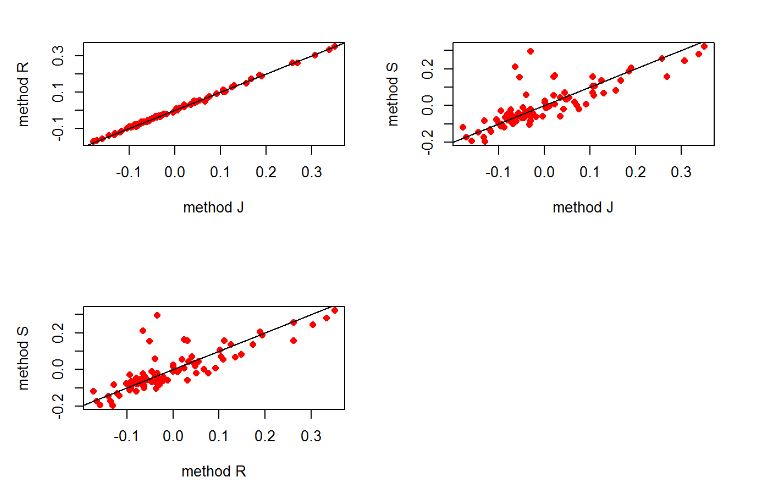
\includegraphics[width=0.9\linewidth]{images/04-DFbetaplots}
% \caption{}
% \label{fig:04-DFbetaplots}
\end{figure}

In the first of the three plots (\textit{Top Right}), strong agreement between method J and method R is indicated. The other plots indicate lack of agreement of methods J and R with method S.



If lack of agreement is indicated, a subsequent analysis using a technique proposed by Roy(2009) can be used to identify the specific cause for this lack of agreement (see next section).
\newpage

The Pearson Correlation coefficient of the DFBetas can be used in conjection with this analysis. A high correlation confirms good agreement. No threshold value for agreement is suggested, and analysts are advised to perform model diagnostics regardless of the correlation coeffient. 


The Bonferroni Outlier Test and Cook's Distance values can be used to identify unusual cases, when the relationship between sets of dfbeta is modelled as a (classical) linear model. In this model, the covariates should be homoskedastic. A test for non-constant variance may be used to verify this. These diagnostic procedures are implementable using the \textbf{\textit{car}} R package.
 
Deming Regression can be used to verify the line of equality. Significance test for Deming regression estimates are not available, but 95\% bootstrap confidence intervals for the slope estimate and intercept estimates can be computed. 


Additionally a mean difference plot can be used to identify outliers. This mean-difference plot differs from the Bland-Altman plot in that the plot is denominated in terms of dfbeta values, and not in measurement units.

If lack of agreement is indicated between methods of measurement, use of Roy's Testing is advised (This is the subject of the next section).
\begin{figure}[h1]
\centering
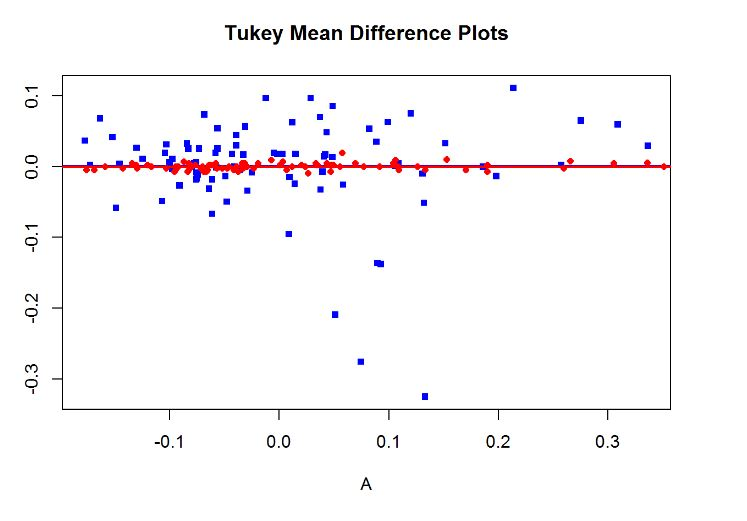
\includegraphics[width=0.7\linewidth]{images/04-TMDplot}
\caption{}
\label{fig:04-TMDplot}
\end{figure}
\newpage
 %========================================================= %
%% - Part E
\subsection*{5. Using Roy's Test to Identify cause of Lack of agreement}

Barnhart specifies three conditions for method of measurement that are required for two methods of measurement to be considered in agreement.

\begin{itemize}
\item[(i)] No Significant Inter-method bias
\item[(ii)] No significant Difference in Within-Subject Variance
\item[(iii)] No significant Difference in Within-Subject Variance 
\end{itemize}
  

Roy(2009) demonstrates a LME model specification, and a series of tests that look at each of these agreement criteria individually. If two methods of measuement lack agreement, the specific reason or reasons for this lack of agreement can be identified.


Roy proposes an LME model with Kronecker product covariance structure in a doubly multivariate setup. Response for $i$th subject can be written as
\[ y_i = \beta_0 + \beta_1x_{i1} + \beta_2x_{i2} + b_{1i}z_{i1}  + b_{2i}z_{i2} + \epsilon_i \]
\begin{itemize}
	\item $\beta_1$ and $\beta_2$ are fixed effects corresponding to both methods. ($\beta_0$ is the intercept.)
	\item $b_{1i}$ and $b_{2i}$ are random effects corresponding to both methods.
\end{itemize}

Overall variability between the two methods ($\Omega$) is sum of between-subject ($D$) and within-subject variability ($\Sigma$),
\[
\mbox{Block } \boldsymbol{\Omega}_i = \left[ \begin{array}{cc} d^2_1 & d_{12}\\ d_{12} & d^2_2\\ \end{array} \right]
+ \left[\begin{array}{cc} \sigma^2_1 & \sigma_{12}\\ \sigma_{12} & \sigma^2_2\\ \end{array}\right].
\]
%============================================== %
%- F:
\subsection*{6. Using Roy's Model to Compute LoAs and CR }

In this short section, a demonstration of how Roy's technique can be used to compute two common MCS metrics: Limits of Agreement and the Coefficient of Repeatabilty. While Limits of Agreement are not used in the analysis proposed here, they are ubiquituous in literature, and a demonstration on how to compute them with the Roy Model would assist the adoption of this proposed method.

The coefficient of repeatability is encountered in Gage R \& R analysis. \textit{(A future exploration of how LME models can be used in that field would be of interest. This is something to include in the Conclusions Section).}
%============================================== %
%- G:
\subsection*{7. Model Diagnostics for Roy's Models}

Further to previous work, this section revisits case-deletion and residual diagnostics, and explores how approaches devised by  Galecki \& Burzykowski (2013) can be used to appraise Roy's model. These authors specifically look at Cook's Distances and Likelihood Distances.
For the Roy Model, Cook's Distances may also be generated using the \textbf{\textit{predictmeans}}



\begin{figure}[h!]
\centering
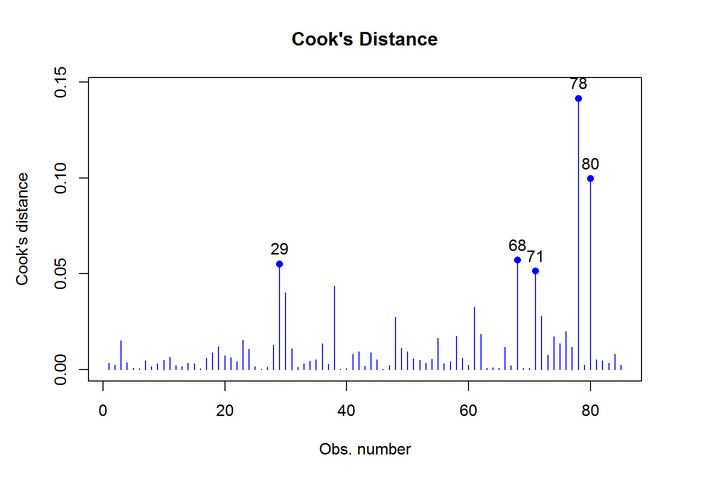
\includegraphics[width=0.7\linewidth]{images/CooksDistancePlot-JS-Roy}
\caption{}
\label{fig:CooksDistancePlot-JS-Roy}
\end{figure}

\begin{figure}[h!]
\centering
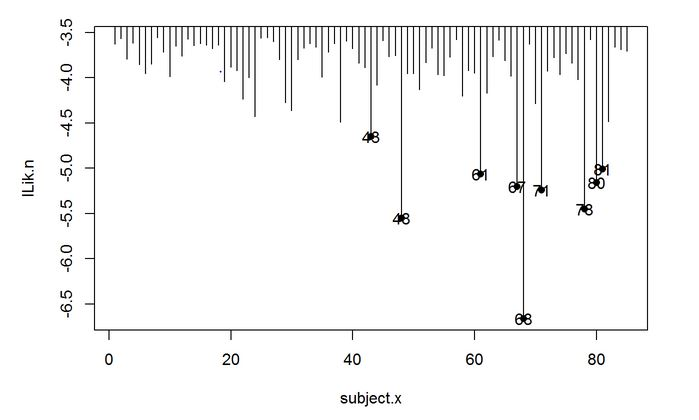
\includegraphics[width=0.7\linewidth]{images/LogLik-JS-Roy}
\caption{}
\label{fig:LogLik-JS-Roy}
\end{figure}

As the model is structurally different from the models discussed in the earlier sections, Residual analysis will be briefly revisited.
\begin{figure}[h!]
\centering
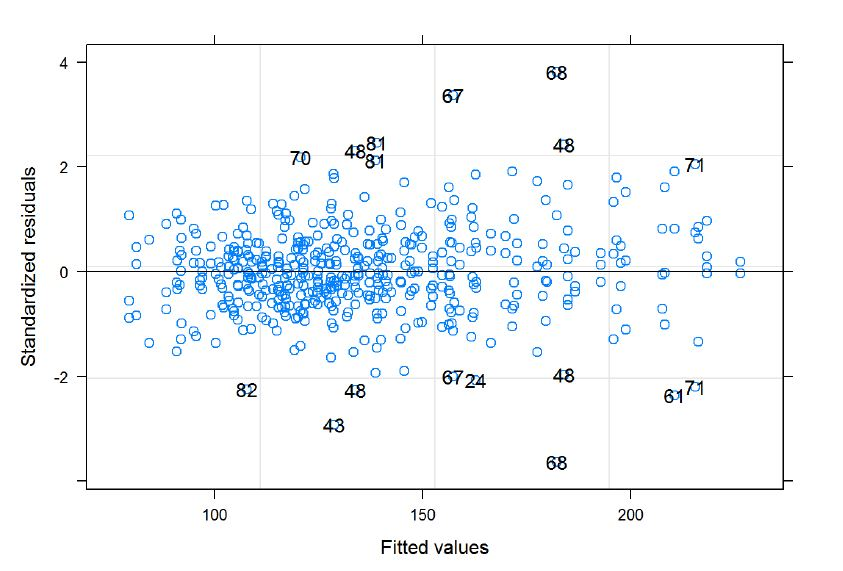
\includegraphics[width=0.7\linewidth]{images/Residuals-JS-Roy}
\caption{}
\label{fig:Residuals-JS-Roy}
\end{figure}

\newpage
\subsection*{8. Case Deletion Diagnostics for the Variance Ratios}
%- H Case Deletion Diagnostics 

Schabenberger advises on the use of deletion diagnostics for variance components of an LME model.
Taking the core principals of his methods, and applying them to the Method Comparison problem, case deletion diagnostics are used on the variance components of the Roy model., specifically the ratio of between subject variances and the within subject covariances respecitvely.


\[ \mbox{BSVR} = \frac{\sigma^2_2}{\sigma^2_2} \phantom{makespace}  \mbox{WSVR} = \frac{d^2_2}{d^2_2} \]

These variance ratios are re-computed for each case removed, and may be analysed seperately or jointly for outliers. 

The Grubbs' Test for Outliers is a commonly used technique for assessing outlier in a univariate data set. As there may be several outliers (i.e. influential cases) present, the Grubbs test is not practical. However outlier detection using to Tukey's 
specification for boxplots (i.e. greater than $Q_3 +1.5 IQR$ or less than $Q_1 - 1.5 IQR$), will suffice. Ranking the asbolute values of the standardizaed scores can also can be used to identify influential cases, even if the data is not normally distributed.

Bivariate Analyses may be applied jointly to the both sets of data sets, e.g Mahalanobis distances. The Mahalanobis distance, while not an intuitive measure in the context of the data, can be used to rank highly influential cases. 

%============================================== %
% - I: 
\subsection*{9. Permutation Test, Power Tests and Missing Data }

This section explores topics such as dependent variable simulation and power analysis, introduced by Galecki \& Burzykowski (2013), and implementable with their \textbf{\textit{nlmeU}} \texttt{R} package.
Using the \textbf{\textit{predictmeans}} \texttt{R} package, it is possible to perform permutation t-tests for coefficients of (fixed) effects and permutation F-tests.

The matter of missing data has not been commonly encountered in either Method Comparison Studies or Linear Mixed Effects Modelling. However Roy (2009) deals with the relevant assumptions regrading missing data. Galecki \& Burzykowski (2013) approaches the subject of missing data in LME Modelling. The \textbf{\textit{nlmeU}} package includes the \texttt{patMiss} function, which ``\textit{allows to compactly present pattern of missing data in a given vector/matrix/data
frame or combination of thereof}".


%================================================%

\subsection*{10. Useful R commands }
This section lists some of the useful \texttt{R} commannds for lme4 and nlme models. It may be moved to the appendices in later editions.


%============================================================%
\end{document}